\section{Measurement}\label{sec:measurement}
\subsection{Redshift-space distortions and AP mapping}
Peculiar velocities can change the genus amplitude even in linear theory \citep{Matsubara1996IsodensityRedshift}. We adopt the plane-parallel approximation with the $z$-axis as the line of sight. To first order in $v_\parallel/c$ \citep{DavisScrimgeour2014Peculiar}, the redshift-space position in the simulation cosmology is
\begin{equation}
s_\parallel=x_\parallel+\frac{(1+z)v_\parallel}{100E(z;\theta_{\mathrm{sim}})},
\end{equation}
where $x_\parallel$ is the comoving position in $h^{-1}\mathrm{Mpc}$, $v_\parallel$ is the peculiar velocity in $\mathrm{km\,s^{-1}}$, and $E=H/H_0$. For the flat, constant-$w$ model used here,
\begin{equation}
E^2(z;\theta)=\Omega_m(1+z)^3+(1-\Omega_m)(1+z)^{3(1+w)}.
\end{equation}

We then apply the AP mapping to the redshift-space positions and box lengths for each scan cosmology $\theta=(\Omega_m,w)$, keeping $h$ fixed \citep{Zunckel2011TopologyDE}:
\begin{equation}
\begin{aligned}
s_\perp^{\mathrm{scan}}&=\alpha_\perp s_\perp^{\mathrm{sim}},\\
s_\parallel^{\mathrm{scan}}&=\alpha_\parallel s_\parallel^{\mathrm{sim}},
\end{aligned}
\end{equation}
\begin{equation}
\begin{aligned}
\alpha_\perp&=\frac{D_M(z;\theta)}{D_M(z;\theta_{\mathrm{sim}})},\\
\alpha_\parallel&=\frac{E(z;\theta_{\mathrm{sim}})}{E(z;\theta)}.
\end{aligned}
\end{equation}
Here $D_M$ is the transverse comoving distance \citep{Hogg1999Distances}. The scaling factors are evaluated at the redshift of each snapshot and applied uniformly within that snapshot. Objects displaced beyond a box face are returned through the opposite face after AP rescaling. The subsequent CIC deposition and genus measurement use open boundaries.

\subsection{Density field and foreground cuts}
We construct the H\,I mass-weighted density field using cloud-in-cell (CIC) interpolation. We fix the target cell size at $\Delta_0=4\,h^{-1}\mathrm{Mpc}$ with $n_i\simeq L_i/\Delta_0$ for the AP-rescaled box lengths $L_i$. We conserve deposited mass at the open box boundary and Fourier transform a zero-extended density contrast (Appendix~\ref{app:implementation}). We correct for the CIC window \citep{Jing2005} and apply Gaussian smoothing with $R=20\,h^{-1}\mathrm{Mpc}$ in scan coordinates.

The cosmological 21-cm signal is much fainter than Galactic and extragalactic radio foregrounds. Their relatively smooth frequency spectra concentrate contamination at low $|k_\parallel|$, corresponding to slowly varying structure along the line of sight. A chromatic instrumental response mixes angular and frequency structure, extending contamination into a wedge at low $|k_\parallel|$ and increasing $k_\perp$ \citep{Datta2010BrightSourceWedge,Morales2012ForegroundShapes,SeoHirata2016Wedge}. Foreground avoidance therefore removes cosmological modes together with the contaminated modes.

To isolate the effect of this anisotropic mode loss, we consider three treatments: no foreground cut (noFG), a horizontal cut removing $|k_\parallel|<0.1\,h\,\mathrm{Mpc}^{-1}$, and the horizontal cut combined with a wedge removing $|k_\parallel|\le m k_\perp$. These masks represent the two characteristic geometries of foreground loss: removal of low line-of-sight modes and the additional angular--frequency mixing of an interferometer. They are controlled, idealized treatments, rather than transfer functions calibrated for a particular survey. Both cuts are defined in scan coordinates, with $k_\parallel=k_z$ and $k_\perp=(k_x^2+k_y^2)^{1/2}$. We keep their parameters fixed across redshifts and scan cosmologies and consider eleven slopes spanning $0.294\le m\le1.692$ (Section~\ref{sec:wedgeareas}). We inverse Fourier transform the filtered field and retain the original box region.

The radial cut can be related to a spectral scale through the local frequency--distance conversion. With $\nu_{\rm obs}=\nu_{21}/(1+z)$ and $\mathrm{d}\chi/\mathrm{d}z=c/H(z)$, its absolute Jacobian is
\begin{equation}\label{eq:frequency_distance}
Y(z)\equiv\left|\frac{\mathrm{d}\chi}{\mathrm{d}\nu_{\rm obs}}\right|
=\frac{c(1+z)^2}{H(z)\nu_{21}}.
\end{equation}
For a spectral mode $\exp(2\pi i\eta\nu_{\rm obs})$, $|k_\parallel|=2\pi|\eta|/Y$. An idealized loss of modes with $|\eta|<\eta_{\rm cut}$ therefore corresponds to
\begin{equation}\label{eq:kcut_frequency}
k_{\rm cut}(z)=\frac{2\pi\eta_{\rm cut}}{Y(z)}
=\frac{2\pi H(z)\nu_{21}}{c(1+z)^2\Delta\nu_{\rm cut}},
\end{equation}
where $\Delta\nu_{\rm cut}=\eta_{\rm cut}^{-1}$ is a spectral period, not a channel width \citep{SeoHirata2016Wedge}. These expressions give wavenumbers in $\mathrm{Mpc}^{-1}$ when $Y$ is in $\mathrm{Mpc}\,\mathrm{MHz}^{-1}$ and frequencies are in MHz; the numerical value in $h\,\mathrm{Mpc}^{-1}$ is obtained by dividing by $h$. A cleaning or instrumental model is needed to specify $\eta_{\rm cut}$. Our fixed $0.1\,h\,\mathrm{Mpc}^{-1}$ is an adopted mode-loss threshold, not a value uniquely derived from the snapshots or $R$. Further scale and wedge relations are given in Appendix~\ref{app:kcut}.

Fig.~\ref{fig:foregroundmask} illustrates the retained and removed modes for the cases used in the field and genus comparisons. Increasing $m$ removes more modes at fixed $k_\perp$, but the wedge adds to the horizontal cut only where $m k_\perp>0.1\,h\,\mathrm{Mpc}^{-1}$. The overlaid Gaussian transfer contours show why the effect of this extra removal also depends on the smoothing scale: modes far from the origin are already strongly attenuated.

\begin{figure*}
\centering
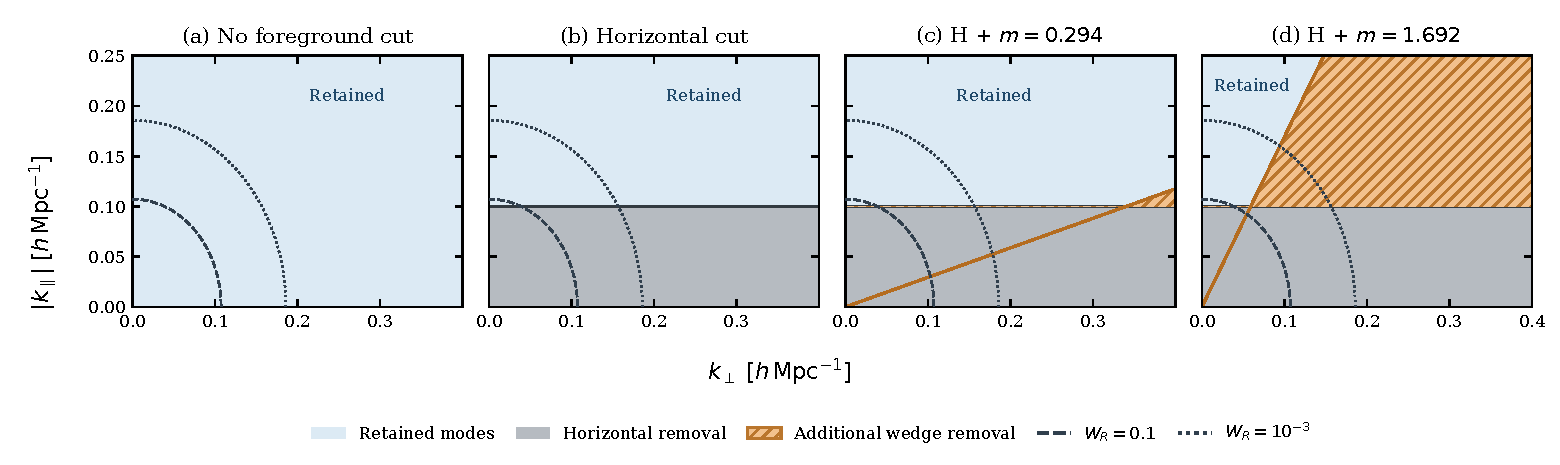
\includegraphics[width=\textwidth]{figures/fig__foreground_kspace.pdf}
\caption{Foreground masks in scan-coordinate Fourier space. Blue marks retained modes, grey the horizontal removal $|k_\parallel|<0.1\,h\,\mathrm{Mpc}^{-1}$, and orange hatching the additional wedge removal. Only $|k_\parallel|\ge0$ is shown; the masks are symmetric in $k_\parallel$. Dashed and dotted arcs indicate the field-amplitude transfer $W_R(k)=\exp[-k^2R^2/2]$ at 0.1 and $10^{-3}$, respectively, for $R=20\,h^{-1}\mathrm{Mpc}$. The diagram shows analytic mask geometry, not a measured power spectrum.}\label{fig:foregroundmask}
\end{figure*}

\subsection{Genus}
The genus describes the connectivity of isodensity surfaces: it distinguishes a network rich in tunnels from isolated high-density regions or enclosed low-density cavities \citep{Hamilton1986Topology,Park2005SDSS}. For the excursion set $E=\{\boldsymbol{x}:\delta(\boldsymbol{x})>\delta_t\}$, we use the cosmological convention $g=-\chi(E)/V$, where $\chi$ is its Euler characteristic and $V$ is the sample volume. Positive genus indicates an excess of tunnels over disconnected components and cavities. We label the density threshold $\delta_t$ by the volume-fraction variable $\nu_f$, defined through
\begin{equation}\label{eq:volumefraction}
f_V(>\delta_t)=\frac{1}{\sqrt{2\pi}}\int_{\nu_f}^{\infty}e^{-u^2/2}\,\mathrm{d}u.
\end{equation}
Thus $\nu_f=0$ selects the upper half of the field volume; it is a Gaussian-equivalent rank threshold, not generally $\delta_t/\sigma$. Comparing fields at fixed $\nu_f$ removes changes caused solely by a uniform positive rescaling of the density contrast \citep{Matsubara2003SmoothedFields}.

In this work, we use 41 equally spaced values over $-2.5\le\nu_f\le2.5$ and determine the corresponding density thresholds separately for each field. We obtain the Euler characteristic from alternating grid-element counts \citep{SchmalzingBuchert1997Morphology}:
\begin{equation}
g(\nu_f)=-\frac{\chi(\nu_f)}{V},\qquad \chi=N_0-N_1+N_2-N_3.
\end{equation}
Here $N_0$, $N_1$, $N_2$ and $N_3$ count vertices, edges, faces and cubes of the excursion set. We use open boundaries, normalize by $V=L_xL_yL_z$ and apply no boundary correction; the counting convention is specified in Appendix~\ref{app:implementation}.

To summarize the amplitude evolution, we fit the Gaussian genus template \citep{Matsubara2003SmoothedFields,Wang2012TopologyGravity}
\begin{equation}
g_{\mathrm{fit}}(\nu_f)=A(1-\nu_f^2)e^{-\nu_f^2/2}
\end{equation}
to the measured curve by equal-weight least squares over $-2.5\le\nu_f\le2.5$. We report the dimensionless amplitude $AR^3$, where $R$ is the Gaussian smoothing scale.
